\documentclass[12pt, a4paper]{article}
\usepackage{../../../myconfig} % Gọi file cấu hình từ ngoài gốc vào
% ==========================================
% BẮT ĐẦU NỘI DUNG TÀI LIỆU
% ==========================================
\begin{document}

% Truyền 3 tham số: {Nhãn cam} {Chữ to chính giữa} {Chữ ở góc phải Header}
\titlebox{Chủ đề: Tích phân}{Ứng dung tích phân tính thể tích hình phẳng thực tế}{Nguyên hàm - Tích phân: Ứng dụng}

\drawdashlines{27}

\questionShortAnswer{15}{1}{Chuẩn bị cho đêm hội diễn văn nghệ chào đón năm mới, nhóm bạn Lan đã làm một chiếc mũ "cách điệu" cho ông già Noel có dáng một khối tròn xoay. Mặt cắt qua trục của chiếc mũ như hình vẽ bên dưới. Biết rằng \( OO' = 6cm \), \( OA = 10cm \), \( OB = 20cm \), đường cong \( AB \) là một phần của parabol có đỉnh là điểm \( B \). Tính thể tích của chiếc mũ (làm tròn đến hàng đơn vị).

\begin{center}
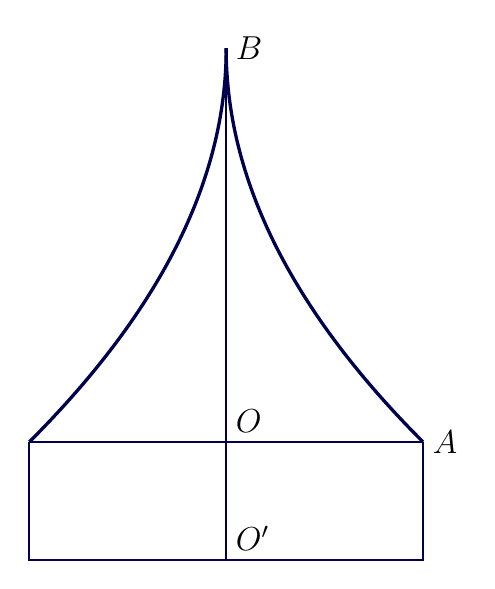
\begin{tikzpicture}[scale=0.25, >=latex]

    \coordinate (O)  at (0, 0);
    \coordinate (O1) at (0, -6); % O'
    \coordinate (A)  at (10, 0);
    \coordinate (A1) at (-10, 0);
    \coordinate (B)  at (0, 20);
    \coordinate (C)  at (10, -6);
    \coordinate (C1) at (-10, -6);

    % 2. Vẽ phần hình chữ nhật phía dưới (khối trụ)
    \draw[thick, blue!30!black] (A1) -- (C1) -- (C) -- (A);

    % 3. Vẽ trục dọc B-O-O' và đoạn ngang A'-O-A
    \draw[thick, blue!30!black] (B) -- (O1);
    \draw[thick, blue!30!black] (A1) -- (A);

    % 4. Vẽ hai đường cong parabol đỉnh B (y = 20 - 0.2*x^2)
    % Cung bên phải từ B(0,20) đến A(10,0)
    \draw[very thick, blue!30!black, domain=0:20, samples=100,variable=\y] 
    plot ( {0.025*\y*\y -\y +10},\y);

    \draw[very thick, blue!30!black, domain=0:20, samples=100,variable=\y] 
    plot ( {-0.025*\y*\y +\y -10},\y);

    % 5. Đánh dấu và nhãn các điểm B, O, O', A
    \node[right, font=\large] at (B)  {$B$};
    \node[above right, font=\large] at (O)  {$O$};
    \node[above right, font=\large] at (O1) {$O'$};
    \node[right, font=\large] at (A)  {$A$};

\end{tikzpicture}
\end{center}
}


\questionShortAnswer{15}{2}{Một khối tròn xoay được tạo thành khi quay hình phẳng \( (H) \) (phần màu xám trong hình vẽ) quanh trục \( AB \).

Miền \( (H) \) được giới hạn bởi đường tròn đường kính \( AB \) và cung tròn tâm \( A \). Biết \( AB = 8 \, \text{cm} \) và điểm \( K \) trong hình vẽ thỏa mãn \( AK = 3 \, \text{cm} \). Thể tích của khối tròn xoay đó bằng bao nhiêu \( \text{cm}^3 \) (làm tròn kết quả đến hàng đơn vị).

\begin{center}
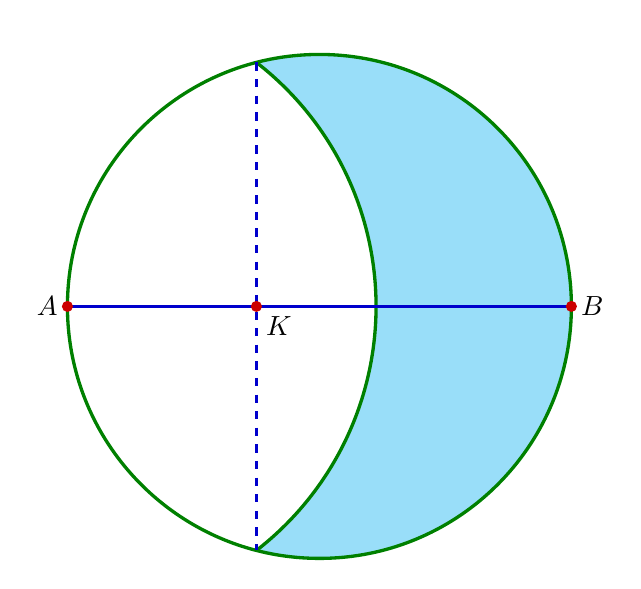
\begin{tikzpicture}[scale=0.8, >=latex]

    % 1. Định nghĩa các thông số hình học
    % Đường kính AB = 8 cm -> Bán kính đường tròn R_circle = 4 cm, Tâm O (0,0)
    % A = (-4, 0), B = (4, 0)
    % AK = 3 cm -> K = (-1, 0)
    % Bán kính cung tròn tâm A là R_arc = AK = 3 cm

    \coordinate (O) at (0, 0);
    \coordinate (A) at (-4, 0);
    \coordinate (B) at (4, 0);
    \coordinate (K) at (-1, 0);
    
    % 2. Tô màu miền (H) (phần lưỡi liềm xanh lam / xám)
    \begin{scope}
        % Vẽ miền tô màu bằng cách kết hợp nửa bên phải đường tròn và trừ đi phần do cung tròn tâm A giới hạn
        \fill[cyan!40] (104.4775:4) arc (104.4775:-104.4775:4) 
            arc (-52.2387:52.2387:4.9) -- cycle;
    \end{scope}

    % 3. Vẽ các đường nét đứt và nét liền
    % Đường tròn chính (đường kính AB, tâm O)
    \draw[very thick, green!50!black] (O) circle (4cm);

    % Cung tròn tâm A bán kính AK = 3cm (được vẽ nét đậm màu xanh)
    \draw[very thick, green!50!black] (-1,3.873) arc (52.2387:-52.2387:4.9);

    % Trục đối xứng AB (nét đậm màu xanh dương)
    \draw[very thick, blue!80!black] (-4, 0) -- (4, 0);  % ĐÃ SỬA

    % Đường thẳng đứng nét đứt qua K
    \draw[dashed, very thick, blue!80!black] (-1, 3.873) -- (-1, -3.873);

    % 4. Đánh dấu các điểm và ghi nhãn
    \fill[red!80!black] (A) circle (2.5pt) node[left, black] {$A$};
    \fill[red!80!black] (B) circle (2.5pt) node[right, black] {$B$};
    \fill[red!80!black] (K) circle (2.5pt) node[below right, black] {$K$};

\end{tikzpicture}
\end{center}
}

% \questionShortAnswer{15}{3}{Một ly thủy tinh có hình dạng phần chứa nước là một hình parabol tròn xoay. Hình dạng này được tạo ra bằng cách quay một phần của đường parabol quanh trục đối xứng của nó. Biết phần chứa nước của ly có chiều cao tính từ đáy ly lên đến miệng ly là \( 10 \, \text{cm} \), đường kính miệng ly là \( 8 \, \text{cm} \) (chỉ tính phần chứa nước, không tính phần thủy tinh).

% Ban đầu, người ta đổ vào ly một lượng nước có thể tích bằng \( \dfrac{1}{4} \) thể tích của ly khi nó chứa đầy nước. Sau đó, người ta đổ thêm vào ly một lượng nước có thể tích bằng với lượng nước đã đổ ban đầu. Hỏi sau khi đổ thêm, chiều cao của mực nước trong ly đã tăng thêm bao nhiêu centimet so với lúc ban đầu (làm tròn đến hàng phần trăm)?

% \begin{center}
% \begin{tikzpicture}[scale=0.35, >=latex]

%     % ==========================================
%     % HÌNH 1: SƠ ĐỒ KÍCH THƯỚC PARABOL (BÊN TRÁI)
%     % ==========================================
%     \begin{scope}[shift={(-16, 0)}]
%         % Parabol lòng ly
%         \draw[thick, black] (-4, 10) parabola bend (0, 0) (4, 10);
        
%         % Miệng ly (Đoạn thẳng)
%         \draw[thick, black] (-4, 10) -- (4, 10);

%         % Trục dọc giữa & đường dóng chiều cao 10cm
%         \draw[<->, >=stealth, black] (0, 0) -- (0, 10);
%         \node[right] at (0.2, 5) {\small $10\text{cm}$};

%         % Kích thước đường kính miệng 8cm
%         \node[above] at (0, 10) {\small $8\text{cm}$};

%     \end{scope}

%     % ==========================================
%     % HÌNH 2: LY NƯỚC BAN ĐẦU - 1/4 THỂ TÍCH (Ở GIỮA)
%     % ==========================================
%     \begin{scope}[shift={(0, 0)}]
%         % Thân ly thủy tinh (bên ngoài)
%         % \draw[thick, black, fill=gray!10] (-4.5, 10.5) 
%         %     parabola bend (0, -0.3) (4.5, 10.5) -- cycle;
            
%         % % Miệng ly thủy tinh
%         % \draw[thick, black, fill=gray!5] (0, 10.5) ellipse (4.5cm and 0.8cm);

%         % Lòng ly
%         \draw[thick, black, fill=purple!5] (-4, 10) 
%             parabola bend (0, 0) (4, 10) ;
%         \draw[thick, black] (0, 10) ellipse (4cm and 0.7cm);

%         % Mực nước h1 = 5cm
%         \draw[thick, black, fill=purple!20] (-2.83, 5) 
%             parabola bend (0, 0) (2.83, 5) -- cycle;
%         \draw[thick, black, fill=purple!30] (0, 5) ellipse (2.83cm and 0.5cm);
%         \draw[dashed, black] (-2.83, 5) arc (180:0:2.83cm and 0.5cm);

%         % Chân ly và đế ly
%         \draw[very thick, red!50!black, fill=red!50!black] (-0.3, 0) -- (-0.3, -4) -- (0.3, -4) -- (0.3, 0) -- cycle;
%         \draw[thick, red!50!black, fill=purple!40] (0, -4) ellipse (3cm and 0.5cm);
%     \end{scope}

%     % ==========================================
%     % HÌNH 3: LY NƯỚC SAU KHI ĐỔ THÊM (BÊN PHẢI)
%     % ==========================================
%     \begin{scope}[shift={(16, 0)}]

%         % Lòng ly
%         \draw[thick, black, fill=purple!5] (-4, 10) 
%             parabola bend (0, 0) (4, 10);
%         \draw[thick, black] (0, 10) ellipse (4cm and 0.7cm);

%         % Mực nước h2 = 7.07cm
%         \draw[thick, black, fill=purple!25] (-3.36, 7.07) 
%             parabola bend (0, 0) (3.36, 7.07) -- cycle;
%         \draw[thick, black, fill=purple!35] (0, 7.07) ellipse (3.36cm and 0.6cm);
%         \draw[dashed, black] (-3.36, 7.07) arc (180:0:3.36cm and 0.6cm);

%         % Chân ly và đế ly
%         \draw[very thick, red!50!black, fill=red!50!black] (-0.3, 0) -- (-0.3, -4) -- (0.3, -4) -- (0.3, 0) -- cycle;
%         \draw[thick, red!50!black, fill=purple!40] (0, -4) ellipse (3cm and 0.5cm);
%     \end{scope}

% \end{tikzpicture}
% \end{center}
% }
% \drawdashlines{35}

\questionShortAnswer{15}{3}{Trong các làng nghề chế tạo đá mỹ nghệ, người ta làm được nhiều đồ trang sức bằng đá rất đẹp. Một người thợ thủ công chế tạo vòng đeo tay hình tròn bằng đá xanh, biết rằng bán kính vòng ngoài của vòng là \( 7cm \), bán kính vòng trong là \( 5cm \) (hình vẽ). Tính thể tích của chiếc vòng (theo đơn vị đo là \( cm^3 \) và làm tròn đến hàng đơn vị).

\begin{figure}[htbp]
    \centering
    \includegraphics[width=0.5\textwidth]{../images/Vong.png}
\end{figure}
}

\newpage
\drawdashlines{35}

\questionShortAnswer{18}{4}{Một bình chứa nước dạng như hình có chiều cao là \(\dfrac{3\pi}{2}\) dm. Nếu lượng nước trong bình có chiều cao là \(x\) (dm) thì mặt nước là hình tròn có bán kính \(\sqrt{2 - \sin x}\) (dm) với \(0 \leq x \leq \dfrac{3\pi}{2}\). Tính dung tích của bình (kết quả làm tròn đến hàng phần trăm của đơn vị đề-xi-mét khối).

\begin{figure}[htbp]
    \centering
    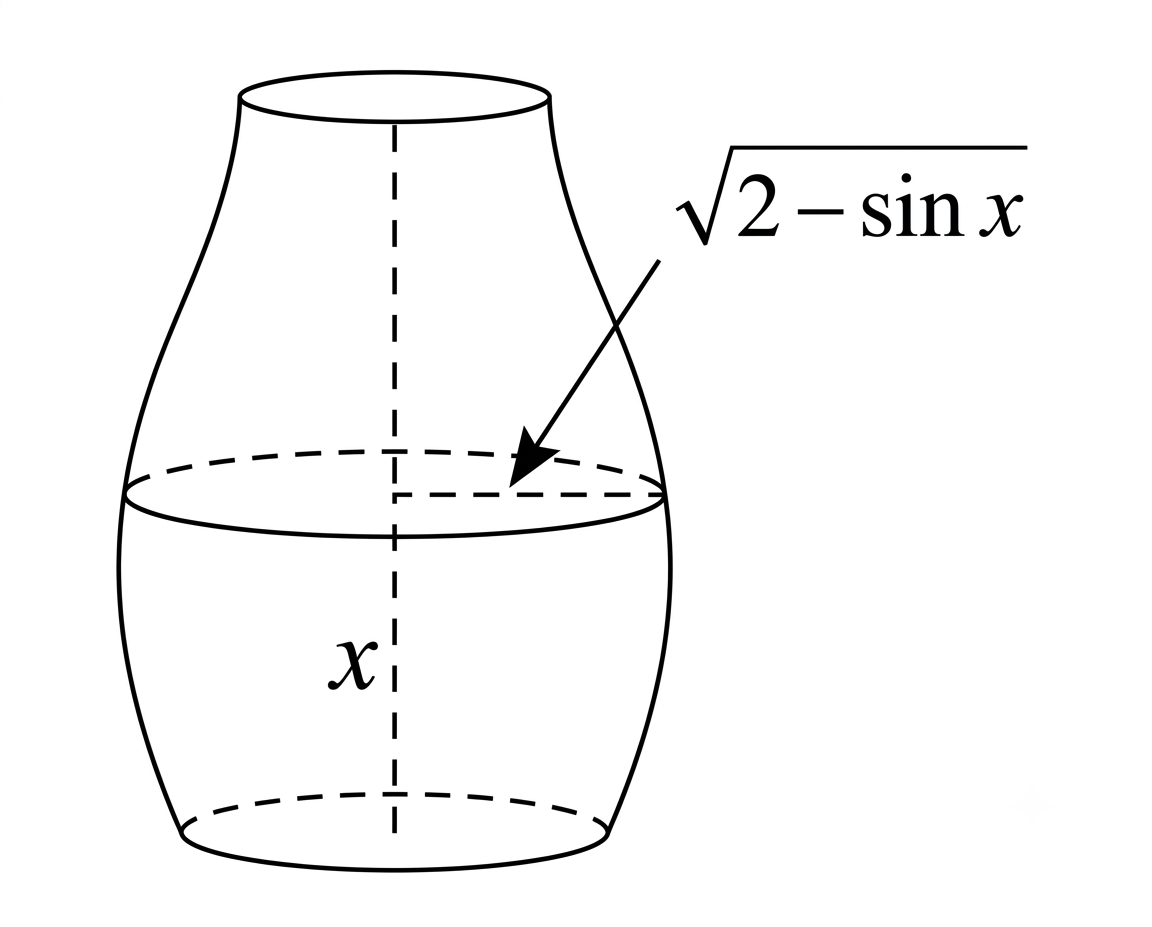
\includegraphics[width=0.4\textwidth]{../images/Lo.png}
\end{figure}

}


\questionShortAnswer{18}{5}{Một cái màn chụp có dạng như hình vẽ bên. Biết rằng mặt cắt của cái màn theo mặt phẳng song song với mặt phẳng đáy và cách mặt đáy một khoảng \( x(m) \), \( 0 \leq x \leq 2 \), là một hình vuông cạnh bằng \( \sqrt{4 - x^2}(m) \). Thể tích của cái màn là bao nhiêu mét khối? (Làm tròn kết quả đến hàng phần mười.)
\begin{figure}[htbp]
    \centering
    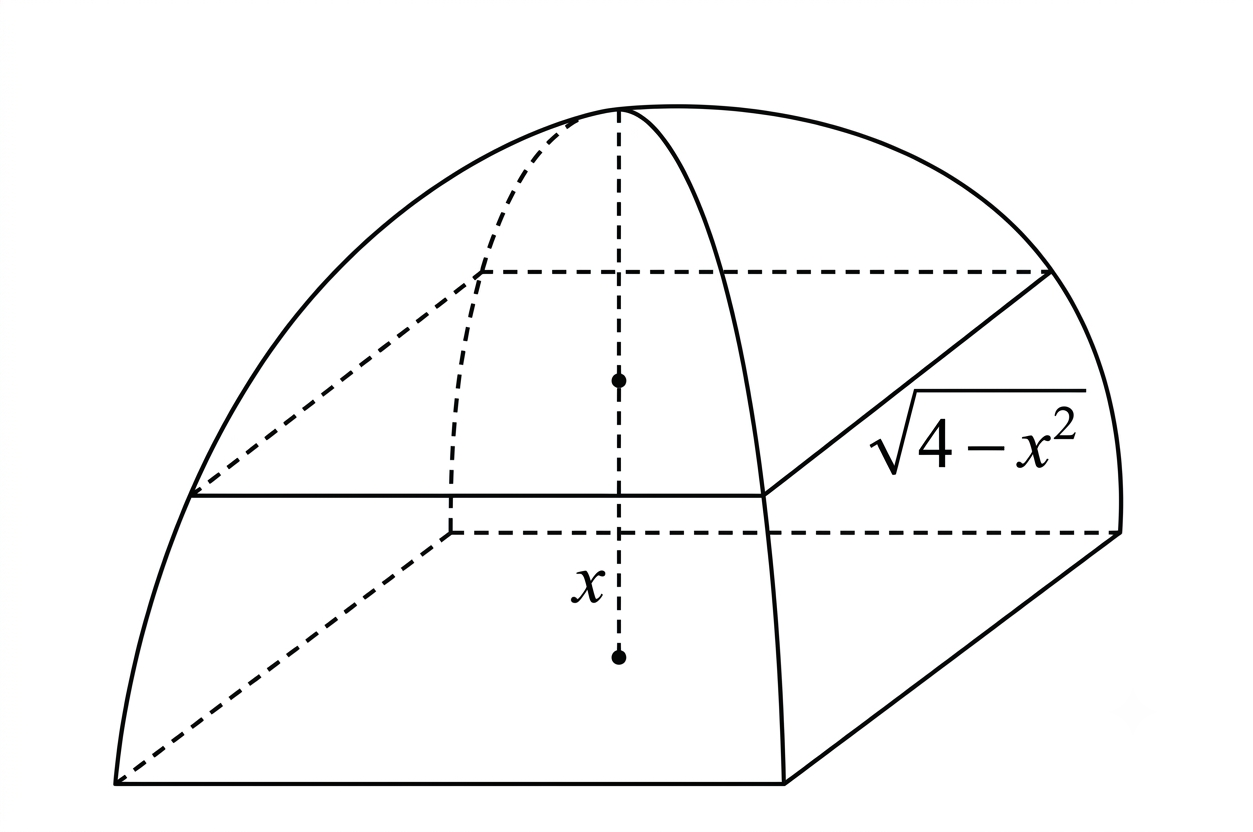
\includegraphics[width=0.5\textwidth]{../images/ManChup.png}
\end{figure}

}


% \questionShortAnswer{15}{7}{Để đặt được một vật trang trí trên mặt bàn, người ta thiết kế một chân đế như sau. Lấy một khối gỗ có dạng khối chóp cụt tứ giác đều với độ dài hai cạnh đáy lần lượt bằng \( 7,4 \, \text{cm} \) và \( 10,4 \, \text{cm} \), bề dày khối gỗ bằng \( 1,5 \, \text{cm} \). Sau đó khoét bỏ đi một phần của khối gỗ sao cho phần đó có dạng vật thể \( H \), ở đó \( H \) nhận được bằng cách cắt khối cầu bán kính \( 5,5 \, \text{cm} \) bởi một mặt phẳng cắt mà mặt cắt là hình tròn bán kính \( 3,5 \, \text{cm} \) (xem hình dưới). 

% \begin{center}
% \begin{tikzpicture}[scale=1, >=latex]

%     % ==========================================
%     % HÌNH 1: KHỐI CHÓP CỤT TÚ GIÁC ĐỀU (BÊN TRÁI)
%     % ==========================================
%     \begin{scope}[shift={(-6.5, 0)}]
%         % Tọa độ đáy lớn (độ dài 10,4 cm)
%         \coordinate (A) at (-2.8, -1.2);
%         \coordinate (B) at (1.8, -1.2);
%         \coordinate (C) at (3.0, 0.4);
%         \coordinate (D) at (-1.6, 0.4);

%         % Tọa độ đáy nhỏ (độ dài 7,4 cm)
%         \coordinate (A1) at (-2.0, 1.6);
%         \coordinate (B1) at (1.2, 1.6);
%         \coordinate (C1) at (2.0, 2.7);
%         \coordinate (D1) at (-1.2, 2.7);

%         % Các cạnh khuất (nét đứt)
%         \draw[thick, dashed, black] (A) -- (D) -- (C);
%         \draw[thick, dashed, black] (D) -- (D1);

%         % Các cạnh nhìn thấy (nét liền)
%         \draw[thick, black] (A) -- (B) -- (C);
%         \draw[thick, black] (A1) -- (B1) -- (C1) -- (D1) -- cycle;
%         \draw[thick, black] (A) -- (A1);
%         \draw[thick, black] (B) -- (B1);
%         \draw[thick, black] (C) -- (C1);

%         % Chiều cao 1,5 cm
%         \coordinate (O_top) at (0, 2.15);
%         \coordinate (O_bot) at (0, -0.4);
        
%         \draw[<->, >=stealth, black] (-0.05, -0.4) -- (-0.05, 2.15);
%         \node[left, font=\small] at (-0.05, 0.8) {$1,5\text{cm}$};

%         % Đường kích thước đáy trên (7,4 cm)
%         \draw[dashed, black] (D1) -- (-1.2, 3.0);
%         \draw[dashed, black] (C1) -- (2, 3.0);
%         \draw[<->, >=stealth, black] (-1.2, 3.1) -- (2, 3.1);
%         \node[above, font=\small] at (0.5, 3.1) {$7,4\text{cm}$};

%         % Đường kích thước đáy dưới (10,4 cm)
%         \draw[dashed, black] (A) -- (-2.8, -1.8);
%         \draw[dashed, black] (B) -- (1.8, -1.8);
%         \draw[<->, >=stealth, black] (-2.8, -1.7) -- (1.8, -1.7);
%         \node[below, font=\small] at (-0.5, -1.7) {$10,4\text{cm}$};
%     \end{scope}

%     % ==========================================
%     % HÌNH 2: KHỐI CẦU VÀ CHỎM CẦU (Ở GIỮA)
%     % ==========================================
%     \begin{scope}[shift={(0, 1.2)}]
%         \pgfmathsetmacro{\R}{2.2} % Bán kính cầu trên hình

%         % Đường tròn lớn của khối cầu
%         \draw[thick, black] (0,0) circle (\R);

%         % Vĩ tuyến xích đạo (nét đứt sau, nét liền trước)
%         \draw[thick, dashed, black] (\R, 0) arc (0:180:\R cm and 0.45cm);
%         \draw[thick, black] (-\R, 0) arc (180:360:\R cm and 0.45cm);

%         % Chỏm cầu (H) ở dưới đáy
%         \begin{scope}
%             \clip (0,0) circle (\R);
%             \fill[cyan!20] (-\R, -1.5) rectangle (\R, -\R);
%         \end{scope}

%         % Đường cắt của chỏm cầu (elip)
%         \draw[thick, black, fill=cyan!15] (0, -1.5) ellipse (1.6cm and 0.35cm);
%         \draw[thick, dashed, black] (-1.6, -1.5) arc (180:0:1.6cm and 0.35cm);

%         % Nhãn (H)
%         \draw[->, >=stealth, black] (-0.8, -2.4) -- (-0.2, -1.9);
%         \node[below left, font=\small\itshape] at (-0.8, -2.2) {$(H)$};
%     \end{scope}

%     % ==========================================
%     % HÌNH 3: HỆ TRỤC TỌA ĐỘ Oxy (BÊN PHẢI)
%     % ==========================================
%     \begin{scope}[shift={(5.5, 1.2)}]
%         \pgfmathsetmacro{\R}{2.2}

%         % Tô màu chỏm cầu (H) bên phải
%         \begin{scope}
%             \clip (0,0) circle (\R);
%             \fill[cyan!20] (1.3, -\R) rectangle (\R, \R);
%         \end{scope}

%         % Hệ trục tọa độ Oxy
%         \draw[->, >=stealth, thick, black] (-2.6, 0) -- (2.8, 0) node[below] {$x$};
%         \draw[->, >=stealth, thick, black] (0, -2.6) -- (0, 2.8) node[right] {$y$};
%         \node[below left, font=\small] at (0, 0) {\small$O$};

%         % Đường tròn R = 5.5
%         \draw[thick, black] (0,0) circle (\R);

%         % Kinh tuyến đứng (nét đứt sau, nét liền trước)
%         \draw[thick,  black] (0, \R) arc (90:270:0.5cm and \R cm);
%         \draw[thick,dashed, black] (0, -\R) arc (-90:90:0.5cm and \R cm);

%         % Mặt cắt hình tròn bán kính 3.5 (ở x = x_cut)
%         \draw[thick,dashed, black] (1.3, 0) ellipse (0.35cm and 1.7cm);
%         \draw[thick, black] (1.3, 1.7) arc (90:270:0.35cm and 1.7cm);

%         % Nhãn giá trị trên trục y (5,5 và 3,5)
%         \node[above left, font=\small] at (0, \R) {$5,5$};
%         \draw[dashed, black] (0, 1.7) -- (1.3, 1.7);
%         \node[left, font=\small] at (0.1, 1.6) {$3,5$};
%         \draw[dashed, black] (1.3, -1.7) -- (1.3, 1.7);

%         % Nhãn (H)
%         \draw[->, >=stealth, black] (2.1, -1.8) -- (1.7, -1.1);
%         \node[below right, font=\small\itshape] at (1.8, -1.7) {$(H)$};
%     \end{scope}

% \end{tikzpicture}
% \end{center}


% Thể tích của khối chân đế bằng bao nhiêu centimét khối (không làm tròn kết quả các phép tính trung gian, chỉ làm tròn kết quả cuối cùng đến hàng phần mười).

% }


% \drawdashlines{35}


% \questionTrueFalse{15}{8}{Một nhà sản xuất muốn thiết kế một hộp đựng kẹo dạng hình tròn xoay gồm hai phần: Phần thứ nhất được tạo thành khi quay "nửa" hình elip quanh một trục; phần thứ hai là nửa hình cầu có bán kính bằng 4 cm. Nếu xét trong hệ trục tọa độ Oxy, đơn vị trên trục là cm thì  
% "nửa" hình elip quay quanh trục Ox để tạo thành phần thứ nhất có phương trình là  
% \(\dfrac{x^2}{64} + \dfrac{y^2}{16} = 1\)  
% với \(-8 \leq x \leq 0\) (xem hình minh họa).
% \begin{figure}[htbp]
%     \centering
%     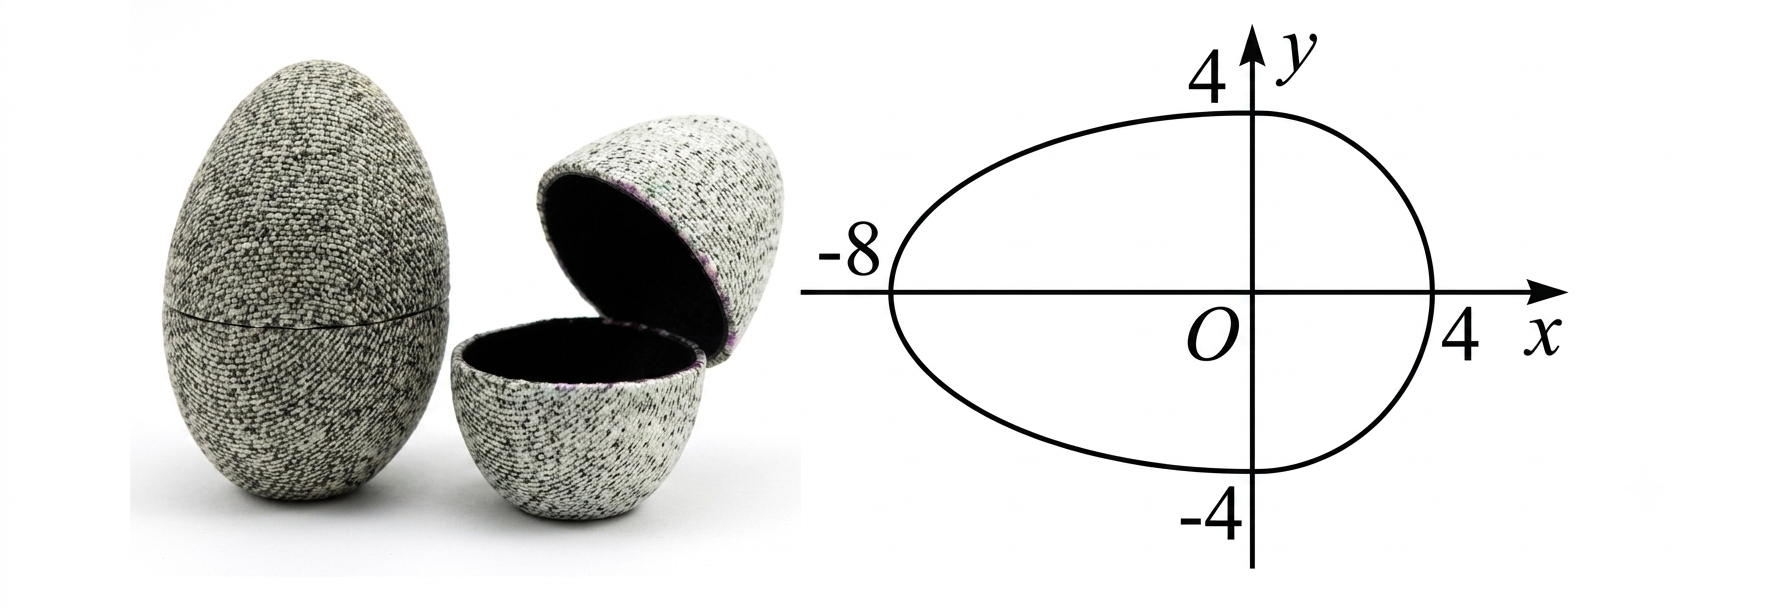
\includegraphics[width=0.5\textwidth]{../images/Trung.png}
% \end{figure}

% }{
%     \textbf{a)} & Thể tích của phần không gian "chứa" trong phần thứ hai (nửa khối cầu) bằng  
%     \(\dfrac{32}{3} \pi \, (\text{cm}^3)\).
%     & \textcolor{amberorange}{$\bigcirc$} & \textcolor{amberorange}{$\bigcirc$} \\ \hline
    
%     \textbf{b)} & Đường thuộc góc phần tư thứ hai trong hệ trục Oxy là đồ thị của hàm số  
%     \(y = \sqrt{16 - \dfrac{x^2}{4}}, \, -8 \leq x \leq 0.\)
%     & \textcolor{amberorange}{$\bigcirc$} & \textcolor{amberorange}{$\bigcirc$} \\ \hline
    
%     \textbf{c)} & Thể tích của phần không gian "chứa" trong phần thứ nhất được tính bởi công thức  
%     \(V = \pi \displaystyle\int_{-8}^{0} \sqrt{16 - \dfrac{x^2}{4}} \, dx \, (\text{cm}^3).\)
%     & \textcolor{amberorange}{$\bigcirc$} & \textcolor{amberorange}{$\bigcirc$} \\ \hline
    
%     \textbf{d)} & Thể tích phần không gian bên trong của hộp đựng kẹo cần thiết kế là \(24\pi \, (\text{cm}^3)\).
%     & \textcolor{amberorange}{$\bigcirc$} & \textcolor{amberorange}{$\bigcirc$} \\
% }


% \drawdashlines{35}

\end {document}
